\subsection{Performance in 2D-Tetris Environments}

\paragraph{Learning dynamics with tetrominoes.}
Figure\ref{fig:train4block} plots the evolution of training score over roughly three thousand episodes for the seven-piece game. Around episode two thousand, the curve exhibits a first pronounced jump, after which successive plateaux and spikes appear. The smoothed trace climbs steadily and stabilises near five thousand, while individual trajectories occasionally exceed 1000000 points, highlighting episodic variance once the agent enters the high-score regime.

\paragraph{Learning dynamics with pentominoes.}
In contrast, Figure\ref{fig:train5block} shows that training on the twelve free pentominoes proceeds far more gradually.  The smoothed score starts around ten and only reaches the high thirteens after fifty thousand episodes.  Raw returns are highly volatile throughout, reflecting the highly variable action space and the difficulty of avoiding self-inflicted holes.  Nevertheless the upward trend is monotonic, suggesting that the curriculum and replay settings still permit meaningful gradient signals even in this more demanding domain.

\paragraph{Test performance.}
Agents trained on tetrominoes finish every test game with scores tightly clustered around 15000. They routinely survive until the board approaches the vertical limit and clear multiple four-line combinations per episode.  By contrast, pentomino agents exhibit pronounced instability: median score is roughly 300, with runs ranging from double digits to slightly above seven hundred.  The policy often top-outs early when confronted with asymmetric shapes such as the \emph{F}, \emph{W}, or \emph{X}.

\paragraph{Discussion.}
The stark contrast between the two curves and their associated test scores highlights how sensitive value-based agents remain to the combinatorial growth of the action space.  While the DQN is able to bootstrap from sparse reward and attain human-level play with classic tetrominoes, the same architecture struggles to generalise to pentominoes despite longer training and identical optimisation hyperparameters. 

\begin{wrapfigure}{r}{0.5\textwidth}
    \centering
    \begin{subfigure}{0.45\textwidth}
        \centering
        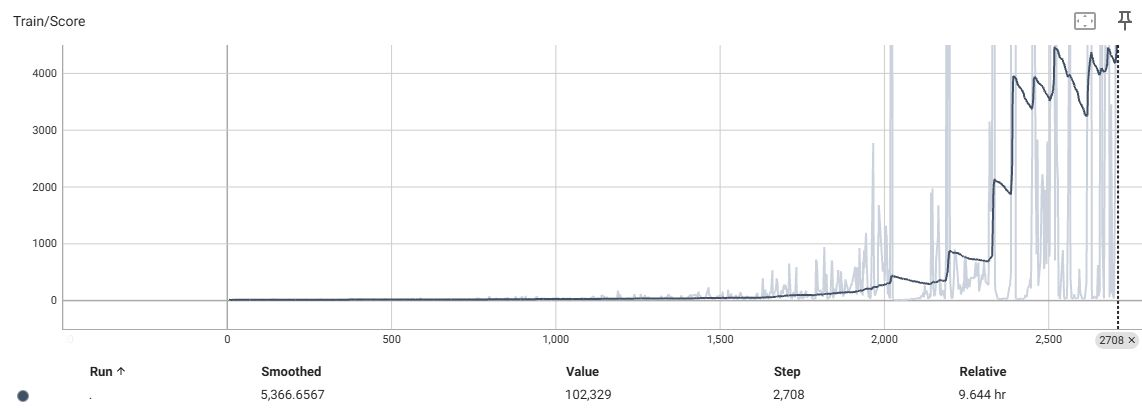
\includegraphics[width=0.90\textwidth]{media/2D_tetramino_training.jpeg}
        \caption{Training curve for 2D-Tetris with Tetraminoes.}
        \label{fig:train4block}
    \end{subfigure}

    \begin{subfigure}{0.45\textwidth}
    \centering
    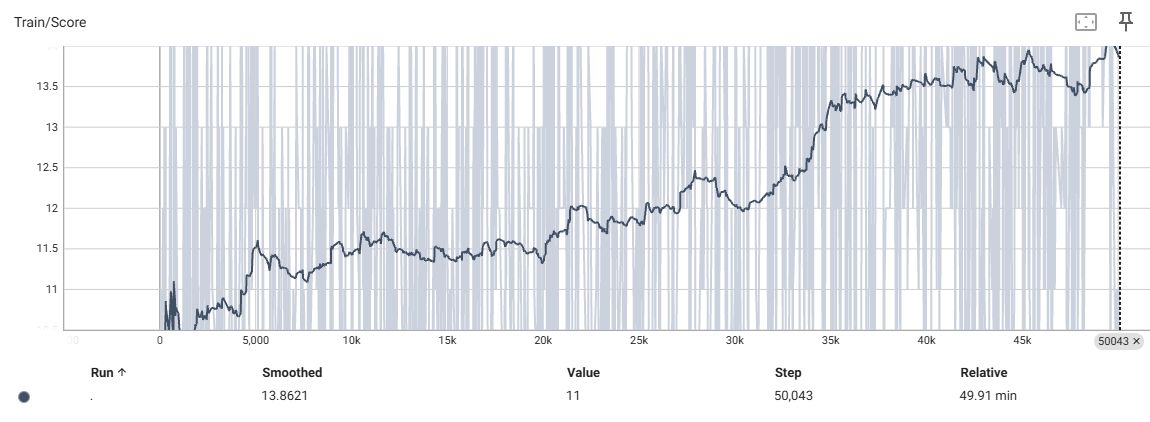
\includegraphics[width=0.90\textwidth]{media/2D_pentamino_training.jpeg}
    \caption{Training curve for 2D-Tetris with Pentominoes.}
    \label{fig:train5block}
    \end{subfigure}

    \caption{The smoothed trace shows the evolution of the average score over the last one hundred episodes, while the raw trace plots the score of each individual episode.}
    \label{fig:2d_training_curves}
\end{wrapfigure}
